\documentclass[1p]{elsarticle_modified}
%\bibliographystyle{elsarticle-num}

%\usepackage[colorlinks]{hyperref}
%\usepackage{abbrmath_seonhwa} %\Abb, \Ascr, \Acal ,\Abf, \Afrak
\usepackage{amsfonts}
\usepackage{amssymb}
\usepackage{amsmath}
\usepackage{amsthm}
\usepackage{scalefnt}
\usepackage{amsbsy}
\usepackage{kotex}
\usepackage{caption}
\usepackage{subfig}
\usepackage{color}
\usepackage{graphicx}
\usepackage{xcolor} %% white, black, red, green, blue, cyan, magenta, yellow
\usepackage{float}
\usepackage{setspace}
\usepackage{hyperref}

\usepackage{tikz}
\usetikzlibrary{arrows}

\usepackage{multirow}
\usepackage{array} % fixed length table
\usepackage{hhline}

%%%%%%%%%%%%%%%%%%%%%
\makeatletter
\renewcommand*\env@matrix[1][\arraystretch]{%
	\edef\arraystretch{#1}%
	\hskip -\arraycolsep
	\let\@ifnextchar\new@ifnextchar
	\array{*\c@MaxMatrixCols c}}
\makeatother %https://tex.stackexchange.com/questions/14071/how-can-i-increase-the-line-spacing-in-a-matrix
%%%%%%%%%%%%%%%

\usepackage[normalem]{ulem}

\newcommand{\msout}[1]{\ifmmode\text{\sout{\ensuremath{#1}}}\else\sout{#1}\fi}
%SOURCE: \msout is \stkout macro in https://tex.stackexchange.com/questions/20609/strikeout-in-math-mode

\newcommand{\cancel}[1]{
	\ifmmode
	{\color{red}\msout{#1}}
	\else
	{\color{red}\sout{#1}}
	\fi
}

\newcommand{\add}[1]{
	{\color{blue}\uwave{#1}}
}

\newcommand{\replace}[2]{
	\ifmmode
	{\color{red}\msout{#1}}{\color{blue}\uwave{#2}}
	\else
	{\color{red}\sout{#1}}{\color{blue}\uwave{#2}}
	\fi
}

\newcommand{\Sol}{\mathcal{S}} %segment
\newcommand{\D}{D} %diagram
\newcommand{\A}{\mathcal{A}} %arc


%%%%%%%%%%%%%%%%%%%%%%%%%%%%%5 test

\def\sl{\operatorname{\textup{SL}}(2,\Cbb)}
\def\psl{\operatorname{\textup{PSL}}(2,\Cbb)}
\def\quan{\mkern 1mu \triangleright \mkern 1mu}

\theoremstyle{definition}
\newtheorem{thm}{Theorem}[section]
\newtheorem{prop}[thm]{Proposition}
\newtheorem{lem}[thm]{Lemma}
\newtheorem{ques}[thm]{Question}
\newtheorem{cor}[thm]{Corollary}
\newtheorem{defn}[thm]{Definition}
\newtheorem{exam}[thm]{Example}
\newtheorem{rmk}[thm]{Remark}
\newtheorem{alg}[thm]{Algorithm}

\newcommand{\I}{\sqrt{-1}}
\begin{document}

%\begin{frontmatter}
%
%\title{Boundary parabolic representations of knots up to 8 crossings}
%
%%% Group authors per affiliation:
%\author{Yunhi Cho} 
%\address{Department of Mathematics, University of Seoul, Seoul, Korea}
%\ead{yhcho@uos.ac.kr}
%
%
%\author{Seonhwa Kim} %\fnref{s_kim}}
%\address{Center for Geometry and Physics, Institute for Basic Science, Pohang, 37673, Korea}
%\ead{ryeona17@ibs.re.kr}
%
%\author{Hyuk Kim}
%\address{Department of Mathematical Sciences, Seoul National University, Seoul 08826, Korea}
%\ead{hyukkim@snu.ac.kr}
%
%\author{Seokbeom Yoon}
%\address{Department of Mathematical Sciences, Seoul National University, Seoul, 08826,  Korea}
%\ead{sbyoon15@snu.ac.kr}
%
%\begin{abstract}
%We find all boundary parabolic representation of knots up to 8 crossings.
%
%\end{abstract}
%\begin{keyword}
%    \MSC[2010] 57M25 
%\end{keyword}
%
%\end{frontmatter}

%\linenumbers
%\tableofcontents
%
\newcommand\colored[1]{\textcolor{white}{\rule[-0.35ex]{0.8em}{1.4ex}}\kern-0.8em\color{red} #1}%
%\newcommand\colored[1]{\textcolor{white}{ #1}\kern-2.17ex	\textcolor{white}{ #1}\kern-1.81ex	\textcolor{white}{ #1}\kern-2.15ex\color{red}#1	}

{\Large $\underline{12a_{0836}~(K12a_{0836})}$}

\setlength{\tabcolsep}{10pt}
\renewcommand{\arraystretch}{1.6}
\vspace{1cm}\begin{tabular}{m{100pt}>{\centering\arraybackslash}m{274pt}}
\multirow{5}{120pt}{
	\centering
	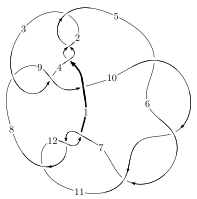
\includegraphics[width=112pt]{../../../GIT/diagram.site/Diagrams/png/1637_12a_0836.png}\\
\ \ \ A knot diagram\footnotemark}&
\allowdisplaybreaks
\textbf{Linearized knot diagam} \\
\cline{2-2}
 &
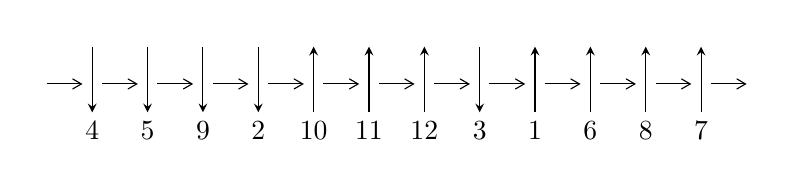
\begin{tikzpicture}[x=20pt, y=17pt]
	% nodes
	\node (C0) at (0, 0) {};
	\node (C1) at (1, 0) {};
	\node (C1U) at (1, +1) {};
	\node (C1D) at (1, -1) {4};

	\node (C2) at (2, 0) {};
	\node (C2U) at (2, +1) {};
	\node (C2D) at (2, -1) {5};

	\node (C3) at (3, 0) {};
	\node (C3U) at (3, +1) {};
	\node (C3D) at (3, -1) {9};

	\node (C4) at (4, 0) {};
	\node (C4U) at (4, +1) {};
	\node (C4D) at (4, -1) {2};

	\node (C5) at (5, 0) {};
	\node (C5U) at (5, +1) {};
	\node (C5D) at (5, -1) {10};

	\node (C6) at (6, 0) {};
	\node (C6U) at (6, +1) {};
	\node (C6D) at (6, -1) {11};

	\node (C7) at (7, 0) {};
	\node (C7U) at (7, +1) {};
	\node (C7D) at (7, -1) {12};

	\node (C8) at (8, 0) {};
	\node (C8U) at (8, +1) {};
	\node (C8D) at (8, -1) {3};

	\node (C9) at (9, 0) {};
	\node (C9U) at (9, +1) {};
	\node (C9D) at (9, -1) {1};

	\node (C10) at (10, 0) {};
	\node (C10U) at (10, +1) {};
	\node (C10D) at (10, -1) {6};

	\node (C11) at (11, 0) {};
	\node (C11U) at (11, +1) {};
	\node (C11D) at (11, -1) {8};

	\node (C12) at (12, 0) {};
	\node (C12U) at (12, +1) {};
	\node (C12D) at (12, -1) {7};
	\node (C13) at (13, 0) {};

	% arrows
	\draw[->,>={angle 60}]
	(C0) edge (C1) (C1) edge (C2) (C2) edge (C3) (C3) edge (C4) (C4) edge (C5) (C5) edge (C6) (C6) edge (C7) (C7) edge (C8) (C8) edge (C9) (C9) edge (C10) (C10) edge (C11) (C11) edge (C12) (C12) edge (C13) ;	\draw[->,>=stealth]
	(C1U) edge (C1D) (C2U) edge (C2D) (C3U) edge (C3D) (C4U) edge (C4D) (C5D) edge (C5U) (C6D) edge (C6U) (C7D) edge (C7U) (C8U) edge (C8D) (C9D) edge (C9U) (C10D) edge (C10U) (C11D) edge (C11U) (C12D) edge (C12U) ;
	\end{tikzpicture} \\
\hhline{~~} \\& 
\textbf{Solving Sequence} \\ \cline{2-2} 
 &
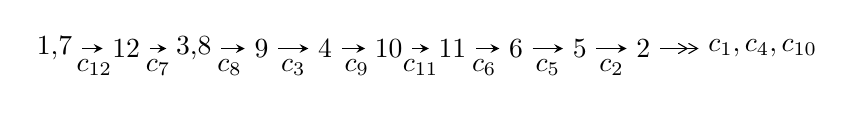
\begin{tikzpicture}[x=23pt, y=7pt]
	% node
	\node (A0) at (-1/8, 0) {1,7};
	\node (A1) at (1, 0) {12};
	\node (A2) at (33/16, 0) {3,8};
	\node (A3) at (25/8, 0) {9};
	\node (A4) at (33/8, 0) {4};
	\node (A5) at (41/8, 0) {10};
	\node (A6) at (49/8, 0) {11};
	\node (A7) at (57/8, 0) {6};
	\node (A8) at (65/8, 0) {5};
	\node (A9) at (73/8, 0) {2};
	\node (C1) at (1/2, -1) {$c_{12}$};
	\node (C2) at (3/2, -1) {$c_{7}$};
	\node (C3) at (21/8, -1) {$c_{8}$};
	\node (C4) at (29/8, -1) {$c_{3}$};
	\node (C5) at (37/8, -1) {$c_{9}$};
	\node (C6) at (45/8, -1) {$c_{11}$};
	\node (C7) at (53/8, -1) {$c_{6}$};
	\node (C8) at (61/8, -1) {$c_{5}$};
	\node (C9) at (69/8, -1) {$c_{2}$};
	\node (A10) at (11, 0) {$c_{1},c_{4},c_{10}$};

	% edge
	\draw[->,>=stealth]	
	(A0) edge (A1) (A1) edge (A2) (A2) edge (A3) (A3) edge (A4) (A4) edge (A5) (A5) edge (A6) (A6) edge (A7) (A7) edge (A8) (A8) edge (A9) ;
	\draw[->>,>={angle 60}]	
	(A9) edge (A10);
\end{tikzpicture} \\ 

\end{tabular} \\

\footnotetext{
The image of knot diagram is generated by the software ``\textbf{Draw programme}" developed by Andrew Bartholomew(\url{http://www.layer8.co.uk/maths/draw/index.htm\#Running-draw}), where we modified some parts for our purpose(\url{https://github.com/CATsTAILs/LinksPainter}).
}\phantom \\ \newline 
\centering \textbf{Ideals for irreducible components\footnotemark of $X_{\text{par}}$} 
 
\begin{align*}
I^u_{1}&=\langle 
- u^{65}+u^{64}+\cdots+b+2 u,\;u^{65}- u^{64}+\cdots+a-2,\;u^{68}-2 u^{67}+\cdots+2 u+1\rangle \\
I^u_{2}&=\langle 
b-1,\;- u^4- u^3-2 u^2+a- u,\;u^6+u^5+3 u^4+2 u^3+2 u^2+u-1\rangle \\
\\
\end{align*}
\raggedright * 2 irreducible components of $\dim_{\mathbb{C}}=0$, with total 74 representations.\\
\footnotetext{All coefficients of polynomials are rational numbers. But the coefficients are sometimes approximated in decimal forms when there is not enough margin.}
\newpage
\renewcommand{\arraystretch}{1}
\centering \section*{I. $I^u_{1}= \langle - u^{65}+u^{64}+\cdots+b+2 u,\;u^{65}- u^{64}+\cdots+a-2,\;u^{68}-2 u^{67}+\cdots+2 u+1 \rangle$}
\flushleft \textbf{(i) Arc colorings}\\
\begin{tabular}{m{7pt} m{180pt} m{7pt} m{180pt} }
\flushright $a_{1}=$&$\begin{pmatrix}1\\0\end{pmatrix}$ \\
\flushright $a_{7}=$&$\begin{pmatrix}0\\u\end{pmatrix}$ \\
\flushright $a_{12}=$&$\begin{pmatrix}1\\u^2\end{pmatrix}$ \\
\flushright $a_{3}=$&$\begin{pmatrix}- u^{65}+u^{64}+\cdots-3 u+2\\u^{65}- u^{64}+\cdots+7 u^2-2 u\end{pmatrix}$ \\
\flushright $a_{8}=$&$\begin{pmatrix}u\\u^3+u\end{pmatrix}$ \\
\flushright $a_{9}=$&$\begin{pmatrix}u^{10}+3 u^8+2 u^6-3 u^4-3 u^2+1\\- u^{10}-4 u^8-5 u^6+3 u^2\end{pmatrix}$ \\
\flushright $a_{4}=$&$\begin{pmatrix}u^{65}- u^{64}+\cdots-4 u+1\\u^{65}- u^{64}+\cdots+4 u^2-3 u\end{pmatrix}$ \\
\flushright $a_{10}=$&$\begin{pmatrix}- u^8-3 u^6-3 u^4+1\\- u^{10}-4 u^8-5 u^6+3 u^2\end{pmatrix}$ \\
\flushright $a_{11}=$&$\begin{pmatrix}u^2+1\\u^4+2 u^2\end{pmatrix}$ \\
\flushright $a_{6}=$&$\begin{pmatrix}- u^5-2 u^3- u\\- u^7-3 u^5-2 u^3+u\end{pmatrix}$ \\
\flushright $a_{5}=$&$\begin{pmatrix}u^{11}+4 u^9+6 u^7+2 u^5-3 u^3-2 u\\u^{13}+5 u^{11}+9 u^9+4 u^7-6 u^5-5 u^3+u\end{pmatrix}$ \\
\flushright $a_{2}=$&$\begin{pmatrix}u^{63}- u^{62}+\cdots-4 u+2\\u^{65}- u^{64}+\cdots+5 u^2-2 u\end{pmatrix}$\\&\end{tabular}
\flushleft \textbf{(ii) Obstruction class $= -1$}\\~\\
\flushleft \textbf{(iii) Cusp Shapes $= -4 u^{67}+8 u^{66}+\cdots+36 u-3$}\\~\\
\newpage\renewcommand{\arraystretch}{1}
\flushleft \textbf{(iv) u-Polynomials at the component}\newline \\
\begin{tabular}{m{50pt}|m{274pt}}
Crossings & \hspace{64pt}u-Polynomials at each crossing \\
\hline $$\begin{aligned}c_{1},c_{2},c_{4}\end{aligned}$$&$\begin{aligned}
&u^{68}-7 u^{67}+\cdots+3 u-1
\end{aligned}$\\
\hline $$\begin{aligned}c_{3},c_{8}\end{aligned}$$&$\begin{aligned}
&u^{68}+u^{67}+\cdots-128 u-64
\end{aligned}$\\
\hline $$\begin{aligned}c_{5},c_{6},c_{10}\end{aligned}$$&$\begin{aligned}
&u^{68}+2 u^{67}+\cdots+172 u+17
\end{aligned}$\\
\hline $$\begin{aligned}c_{7},c_{11},c_{12}\end{aligned}$$&$\begin{aligned}
&u^{68}-2 u^{67}+\cdots+2 u+1
\end{aligned}$\\
\hline $$\begin{aligned}c_{9}\end{aligned}$$&$\begin{aligned}
&u^{68}-6 u^{67}+\cdots+19512 u-3344
\end{aligned}$\\
\hline
\end{tabular}\\~\\
\newpage\renewcommand{\arraystretch}{1}
\flushleft \textbf{(v) Riley Polynomials at the component}\newline \\
\begin{tabular}{m{50pt}|m{274pt}}
Crossings & \hspace{64pt}Riley Polynomials at each crossing \\
\hline $$\begin{aligned}c_{1},c_{2},c_{4}\end{aligned}$$&$\begin{aligned}
&y^{68}-65 y^{67}+\cdots+29 y+1
\end{aligned}$\\
\hline $$\begin{aligned}c_{3},c_{8}\end{aligned}$$&$\begin{aligned}
&y^{68}-39 y^{67}+\cdots-53248 y+4096
\end{aligned}$\\
\hline $$\begin{aligned}c_{5},c_{6},c_{10}\end{aligned}$$&$\begin{aligned}
&y^{68}-66 y^{67}+\cdots-5682 y+289
\end{aligned}$\\
\hline $$\begin{aligned}c_{7},c_{11},c_{12}\end{aligned}$$&$\begin{aligned}
&y^{68}+54 y^{67}+\cdots-26 y+1
\end{aligned}$\\
\hline $$\begin{aligned}c_{9}\end{aligned}$$&$\begin{aligned}
&y^{68}+18 y^{67}+\cdots-465943328 y+11182336
\end{aligned}$\\
\hline
\end{tabular}\\~\\
\newpage\flushleft \textbf{(vi) Complex Volumes and Cusp Shapes}
$$\begin{array}{c|c|c}  
\text{Solutions to }I^u_{1}& \I (\text{vol} + \sqrt{-1}CS) & \text{Cusp shape}\\
 \hline 
\begin{aligned}
u &= \phantom{-}0.274868 + 1.060340 I \\
a &= -0.526754 - 0.257503 I \\
b &= \phantom{-}0.172316 + 0.844015 I\end{aligned}
 & -7.01631 + 3.93719 I & \phantom{-0.000000 } 0 \\ \hline\begin{aligned}
u &= \phantom{-}0.274868 - 1.060340 I \\
a &= -0.526754 + 0.257503 I \\
b &= \phantom{-}0.172316 - 0.844015 I\end{aligned}
 & -7.01631 - 3.93719 I & \phantom{-0.000000 } 0 \\ \hline\begin{aligned}
u &= -0.895864\phantom{ +0.000000I} \\
a &= -0.191061\phantom{ +0.000000I} \\
b &= \phantom{-}0.633345\phantom{ +0.000000I}\end{aligned}
 & \phantom{-}4.93401\phantom{ +0.000000I} & -0.595830\phantom{ +0.000000I} \\ \hline\begin{aligned}
u &= \phantom{-}0.096240 + 1.118240 I \\
a &= \phantom{-}0.850399 - 0.314781 I \\
b &= -0.471781 - 0.369891 I\end{aligned}
 & -1.83195 + 1.81972 I & \phantom{-0.000000 } 0 \\ \hline\begin{aligned}
u &= \phantom{-}0.096240 - 1.118240 I \\
a &= \phantom{-}0.850399 + 0.314781 I \\
b &= -0.471781 + 0.369891 I\end{aligned}
 & -1.83195 - 1.81972 I & \phantom{-0.000000 } 0 \\ \hline\begin{aligned}
u &= \phantom{-}0.869205 + 0.074527 I \\
a &= \phantom{-}1.315300 + 0.517853 I \\
b &= \phantom{-}0.83012 + 1.96876 I\end{aligned}
 & -0.59482 + 10.16420 I & \phantom{-}1.87647 - 5.92631 I \\ \hline\begin{aligned}
u &= \phantom{-}0.869205 - 0.074527 I \\
a &= \phantom{-}1.315300 - 0.517853 I \\
b &= \phantom{-}0.83012 - 1.96876 I\end{aligned}
 & -0.59482 - 10.16420 I & \phantom{-}1.87647 + 5.92631 I \\ \hline\begin{aligned}
u &= -0.861015 + 0.021460 I \\
a &= \phantom{-}0.068130 - 0.155149 I \\
b &= -0.310712 + 0.559057 I\end{aligned}
 & \phantom{-}7.57123 - 1.21218 I & \phantom{-}9.68961 + 0.94684 I \\ \hline\begin{aligned}
u &= -0.861015 - 0.021460 I \\
a &= \phantom{-}0.068130 + 0.155149 I \\
b &= -0.310712 - 0.559057 I\end{aligned}
 & \phantom{-}7.57123 + 1.21218 I & \phantom{-}9.68961 - 0.94684 I \\ \hline\begin{aligned}
u &= \phantom{-}0.856269 + 0.057784 I \\
a &= -1.47487 - 0.56535 I \\
b &= -1.22357 - 1.80577 I\end{aligned}
 & \phantom{-}5.18799 + 5.94447 I & \phantom{-}5.15329 - 5.45502 I\\
 \hline 
 \end{array}$$\newpage$$\begin{array}{c|c|c}  
\text{Solutions to }I^u_{1}& \I (\text{vol} + \sqrt{-1}CS) & \text{Cusp shape}\\
 \hline 
\begin{aligned}
u &= \phantom{-}0.856269 - 0.057784 I \\
a &= -1.47487 + 0.56535 I \\
b &= -1.22357 + 1.80577 I\end{aligned}
 & \phantom{-}5.18799 - 5.94447 I & \phantom{-}5.15329 + 5.45502 I \\ \hline\begin{aligned}
u &= -0.842334 + 0.053972 I \\
a &= -0.054941 + 0.246831 I \\
b &= \phantom{-}0.457743 - 0.884595 I\end{aligned}
 & \phantom{-}2.36110 - 3.67346 I & \phantom{-}3.13855 + 2.67186 I \\ \hline\begin{aligned}
u &= -0.842334 - 0.053972 I \\
a &= -0.054941 - 0.246831 I \\
b &= \phantom{-}0.457743 + 0.884595 I\end{aligned}
 & \phantom{-}2.36110 + 3.67346 I & \phantom{-}3.13855 - 2.67186 I \\ \hline\begin{aligned}
u &= \phantom{-}0.832992 + 0.037249 I \\
a &= \phantom{-}1.70552 + 0.38792 I \\
b &= \phantom{-}1.61773 + 1.11342 I\end{aligned}
 & \phantom{-}3.56303 + 1.00362 I & \phantom{-}2.39038 - 0.55408 I \\ \hline\begin{aligned}
u &= \phantom{-}0.832992 - 0.037249 I \\
a &= \phantom{-}1.70552 - 0.38792 I \\
b &= \phantom{-}1.61773 - 1.11342 I\end{aligned}
 & \phantom{-}3.56303 - 1.00362 I & \phantom{-}2.39038 + 0.55408 I \\ \hline\begin{aligned}
u &= -0.039755 + 1.193740 I \\
a &= -1.47104 + 1.52287 I \\
b &= \phantom{-}1.210760 - 0.091966 I\end{aligned}
 & -4.53839 - 0.93955 I & \phantom{-0.000000 } 0 \\ \hline\begin{aligned}
u &= -0.039755 - 1.193740 I \\
a &= -1.47104 - 1.52287 I \\
b &= \phantom{-}1.210760 + 0.091966 I\end{aligned}
 & -4.53839 + 0.93955 I & \phantom{-0.000000 } 0 \\ \hline\begin{aligned}
u &= \phantom{-}0.726273 + 0.104581 I \\
a &= -1.340580 - 0.221368 I \\
b &= -0.223564 - 0.553926 I\end{aligned}
 & -4.17485 - 0.25355 I & \phantom{-}0.106562 - 0.720449 I \\ \hline\begin{aligned}
u &= \phantom{-}0.726273 - 0.104581 I \\
a &= -1.340580 + 0.221368 I \\
b &= -0.223564 + 0.553926 I\end{aligned}
 & -4.17485 + 0.25355 I & \phantom{-}0.106562 + 0.720449 I \\ \hline\begin{aligned}
u &= \phantom{-}0.139307 + 1.264580 I \\
a &= \phantom{-}0.387719 + 0.377472 I \\
b &= \phantom{-}0.052113 - 0.152925 I\end{aligned}
 & -3.21418 + 2.27728 I & \phantom{-0.000000 } 0\\
 \hline 
 \end{array}$$\newpage$$\begin{array}{c|c|c}  
\text{Solutions to }I^u_{1}& \I (\text{vol} + \sqrt{-1}CS) & \text{Cusp shape}\\
 \hline 
\begin{aligned}
u &= \phantom{-}0.139307 - 1.264580 I \\
a &= \phantom{-}0.387719 - 0.377472 I \\
b &= \phantom{-}0.052113 + 0.152925 I\end{aligned}
 & -3.21418 - 2.27728 I & \phantom{-0.000000 } 0 \\ \hline\begin{aligned}
u &= \phantom{-}0.420834 + 1.201420 I \\
a &= -1.004800 + 0.249172 I \\
b &= \phantom{-}0.82821 - 1.85021 I\end{aligned}
 & -4.06146 - 5.54434 I & \phantom{-0.000000 } 0 \\ \hline\begin{aligned}
u &= \phantom{-}0.420834 - 1.201420 I \\
a &= -1.004800 - 0.249172 I \\
b &= \phantom{-}0.82821 + 1.85021 I\end{aligned}
 & -4.06146 + 5.54434 I & \phantom{-0.000000 } 0 \\ \hline\begin{aligned}
u &= -0.385541 + 1.220900 I \\
a &= -1.264540 - 0.576743 I \\
b &= \phantom{-}0.601184 + 0.839021 I\end{aligned}
 & -1.23320 - 0.73928 I & \phantom{-0.000000 } 0 \\ \hline\begin{aligned}
u &= -0.385541 - 1.220900 I \\
a &= -1.264540 + 0.576743 I \\
b &= \phantom{-}0.601184 - 0.839021 I\end{aligned}
 & -1.23320 + 0.73928 I & \phantom{-0.000000 } 0 \\ \hline\begin{aligned}
u &= \phantom{-}0.402134 + 1.217770 I \\
a &= \phantom{-}1.050320 + 0.234054 I \\
b &= -1.21789 + 1.63529 I\end{aligned}
 & \phantom{-}1.61428 - 1.42992 I & \phantom{-0.000000 } 0 \\ \hline\begin{aligned}
u &= \phantom{-}0.402134 - 1.217770 I \\
a &= \phantom{-}1.050320 - 0.234054 I \\
b &= -1.21789 - 1.63529 I\end{aligned}
 & \phantom{-}1.61428 + 1.42992 I & \phantom{-0.000000 } 0 \\ \hline\begin{aligned}
u &= \phantom{-}0.376637 + 1.240150 I \\
a &= -0.656599 - 1.012060 I \\
b &= \phantom{-}1.64633 - 0.88359 I\end{aligned}
 & -0.15109 + 3.34387 I & \phantom{-0.000000 } 0 \\ \hline\begin{aligned}
u &= \phantom{-}0.376637 - 1.240150 I \\
a &= -0.656599 + 1.012060 I \\
b &= \phantom{-}1.64633 + 0.88359 I\end{aligned}
 & -0.15109 - 3.34387 I & \phantom{-0.000000 } 0 \\ \hline\begin{aligned}
u &= -0.402053 + 1.254660 I \\
a &= \phantom{-}0.816153 + 0.355455 I \\
b &= -0.409003 - 0.522193 I\end{aligned}
 & \phantom{-}3.75268 - 3.31527 I & \phantom{-0.000000 } 0\\
 \hline 
 \end{array}$$\newpage$$\begin{array}{c|c|c}  
\text{Solutions to }I^u_{1}& \I (\text{vol} + \sqrt{-1}CS) & \text{Cusp shape}\\
 \hline 
\begin{aligned}
u &= -0.402053 - 1.254660 I \\
a &= \phantom{-}0.816153 - 0.355455 I \\
b &= -0.409003 + 0.522193 I\end{aligned}
 & \phantom{-}3.75268 + 3.31527 I & \phantom{-0.000000 } 0 \\ \hline\begin{aligned}
u &= -0.104897 + 1.326030 I \\
a &= \phantom{-}0.59543 + 3.16636 I \\
b &= \phantom{-}0.56443 - 1.71708 I\end{aligned}
 & -6.63847 - 0.67362 I & \phantom{-0.000000 } 0 \\ \hline\begin{aligned}
u &= -0.104897 - 1.326030 I \\
a &= \phantom{-}0.59543 - 3.16636 I \\
b &= \phantom{-}0.56443 + 1.71708 I\end{aligned}
 & -6.63847 + 0.67362 I & \phantom{-0.000000 } 0 \\ \hline\begin{aligned}
u &= \phantom{-}0.126734 + 1.333640 I \\
a &= -0.924830 - 0.807120 I \\
b &= \phantom{-}0.106274 + 0.311282 I\end{aligned}
 & -8.45190 + 3.15667 I & \phantom{-0.000000 } 0 \\ \hline\begin{aligned}
u &= \phantom{-}0.126734 - 1.333640 I \\
a &= -0.924830 + 0.807120 I \\
b &= \phantom{-}0.106274 - 0.311282 I\end{aligned}
 & -8.45190 - 3.15667 I & \phantom{-0.000000 } 0 \\ \hline\begin{aligned}
u &= -0.146516 + 1.332920 I \\
a &= -0.99913 - 3.23738 I \\
b &= -0.36801 + 1.96714 I\end{aligned}
 & -6.11073 - 5.54221 I & \phantom{-0.000000 } 0 \\ \hline\begin{aligned}
u &= -0.146516 - 1.332920 I \\
a &= -0.99913 + 3.23738 I \\
b &= -0.36801 - 1.96714 I\end{aligned}
 & -6.11073 + 5.54221 I & \phantom{-0.000000 } 0 \\ \hline\begin{aligned}
u &= -0.427740 + 1.279080 I \\
a &= -0.709037 + 0.446061 I \\
b &= \phantom{-}0.629160 - 0.054561 I\end{aligned}
 & \phantom{-}0.96243 - 4.73147 I & \phantom{-0.000000 } 0 \\ \hline\begin{aligned}
u &= -0.427740 - 1.279080 I \\
a &= -0.709037 - 0.446061 I \\
b &= \phantom{-}0.629160 + 0.054561 I\end{aligned}
 & \phantom{-}0.96243 + 4.73147 I & \phantom{-0.000000 } 0 \\ \hline\begin{aligned}
u &= -0.396517 + 1.289790 I \\
a &= -0.091140 - 0.825123 I \\
b &= -0.217786 + 0.572163 I\end{aligned}
 & \phantom{-}3.48887 - 5.72199 I & \phantom{-0.000000 } 0\\
 \hline 
 \end{array}$$\newpage$$\begin{array}{c|c|c}  
\text{Solutions to }I^u_{1}& \I (\text{vol} + \sqrt{-1}CS) & \text{Cusp shape}\\
 \hline 
\begin{aligned}
u &= -0.396517 - 1.289790 I \\
a &= -0.091140 + 0.825123 I \\
b &= -0.217786 - 0.572163 I\end{aligned}
 & \phantom{-}3.48887 + 5.72199 I & \phantom{-0.000000 } 0 \\ \hline\begin{aligned}
u &= \phantom{-}0.375212 + 1.299320 I \\
a &= \phantom{-}0.99882 - 2.11483 I \\
b &= \phantom{-}1.59088 + 1.31222 I\end{aligned}
 & -0.60813 + 5.34727 I & \phantom{-0.000000 } 0 \\ \hline\begin{aligned}
u &= \phantom{-}0.375212 - 1.299320 I \\
a &= \phantom{-}0.99882 + 2.11483 I \\
b &= \phantom{-}1.59088 - 1.31222 I\end{aligned}
 & -0.60813 - 5.34727 I & \phantom{-0.000000 } 0 \\ \hline\begin{aligned}
u &= \phantom{-}0.325026 + 1.312790 I \\
a &= -1.12164 + 1.07523 I \\
b &= -0.598332 - 0.646888 I\end{aligned}
 & -8.57365 + 3.57514 I & \phantom{-0.000000 } 0 \\ \hline\begin{aligned}
u &= \phantom{-}0.325026 - 1.312790 I \\
a &= -1.12164 - 1.07523 I \\
b &= -0.598332 + 0.646888 I\end{aligned}
 & -8.57365 - 3.57514 I & \phantom{-0.000000 } 0 \\ \hline\begin{aligned}
u &= -0.355477 + 0.540754 I \\
a &= -1.56452 - 0.66386 I \\
b &= \phantom{-}0.109402 + 1.371900 I\end{aligned}
 & -7.83604 + 3.56277 I & -3.48429 - 0.26987 I \\ \hline\begin{aligned}
u &= -0.355477 - 0.540754 I \\
a &= -1.56452 + 0.66386 I \\
b &= \phantom{-}0.109402 - 1.371900 I\end{aligned}
 & -7.83604 - 3.56277 I & -3.48429 + 0.26987 I \\ \hline\begin{aligned}
u &= -0.536593 + 0.355337 I \\
a &= \phantom{-}1.184830 + 0.517192 I \\
b &= \phantom{-}0.32245 - 1.66008 I\end{aligned}
 & -7.14400 - 6.91551 I & -1.34390 + 7.27933 I \\ \hline\begin{aligned}
u &= -0.536593 - 0.355337 I \\
a &= \phantom{-}1.184830 - 0.517192 I \\
b &= \phantom{-}0.32245 + 1.66008 I\end{aligned}
 & -7.14400 + 6.91551 I & -1.34390 - 7.27933 I \\ \hline\begin{aligned}
u &= -0.380136 + 1.310130 I \\
a &= \phantom{-}0.137470 + 1.319400 I \\
b &= \phantom{-}0.338862 - 0.902883 I\end{aligned}
 & -1.90173 - 8.06695 I & \phantom{-0.000000 } 0\\
 \hline 
 \end{array}$$\newpage$$\begin{array}{c|c|c}  
\text{Solutions to }I^u_{1}& \I (\text{vol} + \sqrt{-1}CS) & \text{Cusp shape}\\
 \hline 
\begin{aligned}
u &= -0.380136 - 1.310130 I \\
a &= \phantom{-}0.137470 - 1.319400 I \\
b &= \phantom{-}0.338862 + 0.902883 I\end{aligned}
 & -1.90173 + 8.06695 I & \phantom{-0.000000 } 0 \\ \hline\begin{aligned}
u &= -0.076307 + 1.363730 I \\
a &= -0.76099 - 2.76851 I \\
b &= -0.28084 + 1.50736 I\end{aligned}
 & -13.64730 + 2.32372 I & \phantom{-0.000000 } 0 \\ \hline\begin{aligned}
u &= -0.076307 - 1.363730 I \\
a &= -0.76099 + 2.76851 I \\
b &= -0.28084 - 1.50736 I\end{aligned}
 & -13.64730 - 2.32372 I & \phantom{-0.000000 } 0 \\ \hline\begin{aligned}
u &= -0.165622 + 1.358730 I \\
a &= \phantom{-}1.04285 + 3.06303 I \\
b &= \phantom{-}0.23955 - 1.93117 I\end{aligned}
 & -12.5196 - 9.3121 I & \phantom{-0.000000 } 0 \\ \hline\begin{aligned}
u &= -0.165622 - 1.358730 I \\
a &= \phantom{-}1.04285 - 3.06303 I \\
b &= \phantom{-}0.23955 + 1.93117 I\end{aligned}
 & -12.5196 + 9.3121 I & \phantom{-0.000000 } 0 \\ \hline\begin{aligned}
u &= \phantom{-}0.388285 + 1.314120 I \\
a &= -1.57085 + 2.17185 I \\
b &= -1.20114 - 1.94252 I\end{aligned}
 & \phantom{-}0.89978 + 10.41270 I & \phantom{-0.000000 } 0 \\ \hline\begin{aligned}
u &= \phantom{-}0.388285 - 1.314120 I \\
a &= -1.57085 - 2.17185 I \\
b &= -1.20114 + 1.94252 I\end{aligned}
 & \phantom{-}0.89978 - 10.41270 I & \phantom{-0.000000 } 0 \\ \hline\begin{aligned}
u &= \phantom{-}0.393601 + 1.326560 I \\
a &= \phantom{-}1.80874 - 2.01322 I \\
b &= \phantom{-}0.80659 + 2.06065 I\end{aligned}
 & -4.9810 + 14.6950 I & \phantom{-0.000000 } 0 \\ \hline\begin{aligned}
u &= \phantom{-}0.393601 - 1.326560 I \\
a &= \phantom{-}1.80874 + 2.01322 I \\
b &= \phantom{-}0.80659 - 2.06065 I\end{aligned}
 & -4.9810 - 14.6950 I & \phantom{-0.000000 } 0 \\ \hline\begin{aligned}
u &= -0.461201 + 0.310199 I \\
a &= -1.342820 - 0.347618 I \\
b &= -0.39492 + 1.52052 I\end{aligned}
 & -1.02729 - 3.44858 I & \phantom{-}1.47745 + 8.39807 I\\
 \hline 
 \end{array}$$\newpage$$\begin{array}{c|c|c}  
\text{Solutions to }I^u_{1}& \I (\text{vol} + \sqrt{-1}CS) & \text{Cusp shape}\\
 \hline 
\begin{aligned}
u &= -0.461201 - 0.310199 I \\
a &= -1.342820 + 0.347618 I \\
b &= -0.39492 - 1.52052 I\end{aligned}
 & -1.02729 + 3.44858 I & \phantom{-}1.47745 - 8.39807 I \\ \hline\begin{aligned}
u &= \phantom{-}0.397825 + 0.339088 I \\
a &= -1.159450 - 0.792131 I \\
b &= \phantom{-}0.421810 + 0.207688 I\end{aligned}
 & -3.31331 + 1.34942 I & -0.69445 - 4.81797 I \\ \hline\begin{aligned}
u &= \phantom{-}0.397825 - 0.339088 I \\
a &= -1.159450 + 0.792131 I \\
b &= \phantom{-}0.421810 - 0.207688 I\end{aligned}
 & -3.31331 - 1.34942 I & -0.69445 + 4.81797 I \\ \hline\begin{aligned}
u &= -0.295735 + 0.374812 I \\
a &= \phantom{-}1.64151 + 0.53692 I \\
b &= \phantom{-}0.199141 - 1.171910 I\end{aligned}
 & -1.52842 + 0.74751 I & -1.82763 + 0.40847 I \\ \hline\begin{aligned}
u &= -0.295735 - 0.374812 I \\
a &= \phantom{-}1.64151 - 0.53692 I \\
b &= \phantom{-}0.199141 + 1.171910 I\end{aligned}
 & -1.52842 - 0.74751 I & -1.82763 - 0.40847 I \\ \hline\begin{aligned}
u &= \phantom{-}0.437462 + 0.102734 I \\
a &= \phantom{-}0.720475 + 0.489361 I \\
b &= -0.1275350 - 0.0350142 I\end{aligned}
 & \phantom{-}0.917664 + 0.265375 I & \phantom{-}10.32983 - 1.81252 I \\ \hline\begin{aligned}
u &= \phantom{-}0.437462 - 0.102734 I \\
a &= \phantom{-}0.720475 - 0.489361 I \\
b &= -0.1275350 + 0.0350142 I\end{aligned}
 & \phantom{-}0.917664 - 0.265375 I & \phantom{-}10.32983 + 1.81252 I \\ \hline\begin{aligned}
u &= -0.227060\phantom{ +0.000000I} \\
a &= \phantom{-}2.62077\phantom{ +0.000000I} \\
b &= \phantom{-}0.966677\phantom{ +0.000000I}\end{aligned}
 & -1.29008\phantom{ +0.000000I} & -12.1470\phantom{ +0.000000I}\\
 \hline 
 \end{array}$$\newpage\newpage\renewcommand{\arraystretch}{1}
\centering \section*{II. $I^u_{2}= \langle b-1,\;- u^4- u^3-2 u^2+a- u,\;u^6+u^5+3 u^4+2 u^3+2 u^2+u-1 \rangle$}
\flushleft \textbf{(i) Arc colorings}\\
\begin{tabular}{m{7pt} m{180pt} m{7pt} m{180pt} }
\flushright $a_{1}=$&$\begin{pmatrix}1\\0\end{pmatrix}$ \\
\flushright $a_{7}=$&$\begin{pmatrix}0\\u\end{pmatrix}$ \\
\flushright $a_{12}=$&$\begin{pmatrix}1\\u^2\end{pmatrix}$ \\
\flushright $a_{3}=$&$\begin{pmatrix}u^4+u^3+2 u^2+u\\1\end{pmatrix}$ \\
\flushright $a_{8}=$&$\begin{pmatrix}u\\u^3+u\end{pmatrix}$ \\
\flushright $a_{9}=$&$\begin{pmatrix}u\\u^3+u\end{pmatrix}$ \\
\flushright $a_{4}=$&$\begin{pmatrix}u^4+u^3+2 u^2+u\\1\end{pmatrix}$ \\
\flushright $a_{10}=$&$\begin{pmatrix}u^3+2 u\\u^3+u\end{pmatrix}$ \\
\flushright $a_{11}=$&$\begin{pmatrix}u^2+1\\u^4+2 u^2\end{pmatrix}$ \\
\flushright $a_{6}=$&$\begin{pmatrix}- u^5-2 u^3- u\\- u^5- u^4-2 u^3- u^2- u+1\end{pmatrix}$ \\
\flushright $a_{5}=$&$\begin{pmatrix}-1\\0\end{pmatrix}$ \\
\flushright $a_{2}=$&$\begin{pmatrix}u^4+u^3+2 u^2+u+1\\1\end{pmatrix}$\\&\end{tabular}
\flushleft \textbf{(ii) Obstruction class $= 1$}\\~\\
\flushleft \textbf{(iii) Cusp Shapes $= 5 u^4+6 u^3+11 u^2+6 u+5$}\\~\\
\newpage\renewcommand{\arraystretch}{1}
\flushleft \textbf{(iv) u-Polynomials at the component}\newline \\
\begin{tabular}{m{50pt}|m{274pt}}
Crossings & \hspace{64pt}u-Polynomials at each crossing \\
\hline $$\begin{aligned}c_{1},c_{2}\end{aligned}$$&$\begin{aligned}
&(u-1)^6
\end{aligned}$\\
\hline $$\begin{aligned}c_{3},c_{8}\end{aligned}$$&$\begin{aligned}
&u^6
\end{aligned}$\\
\hline $$\begin{aligned}c_{4}\end{aligned}$$&$\begin{aligned}
&(u+1)^6
\end{aligned}$\\
\hline $$\begin{aligned}c_{5},c_{6},c_{9}\end{aligned}$$&$\begin{aligned}
&u^6+u^5-3 u^4-2 u^3+2 u^2- u-1
\end{aligned}$\\
\hline $$\begin{aligned}c_{7}\end{aligned}$$&$\begin{aligned}
&u^6- u^5+3 u^4-2 u^3+2 u^2- u-1
\end{aligned}$\\
\hline $$\begin{aligned}c_{10}\end{aligned}$$&$\begin{aligned}
&u^6- u^5-3 u^4+2 u^3+2 u^2+u-1
\end{aligned}$\\
\hline $$\begin{aligned}c_{11},c_{12}\end{aligned}$$&$\begin{aligned}
&u^6+u^5+3 u^4+2 u^3+2 u^2+u-1
\end{aligned}$\\
\hline
\end{tabular}\\~\\
\newpage\renewcommand{\arraystretch}{1}
\flushleft \textbf{(v) Riley Polynomials at the component}\newline \\
\begin{tabular}{m{50pt}|m{274pt}}
Crossings & \hspace{64pt}Riley Polynomials at each crossing \\
\hline $$\begin{aligned}c_{1},c_{2},c_{4}\end{aligned}$$&$\begin{aligned}
&(y-1)^6
\end{aligned}$\\
\hline $$\begin{aligned}c_{3},c_{8}\end{aligned}$$&$\begin{aligned}
&y^6
\end{aligned}$\\
\hline $$\begin{aligned}c_{5},c_{6},c_{9}\\c_{10}\end{aligned}$$&$\begin{aligned}
&y^6-7 y^5+17 y^4-16 y^3+6 y^2-5 y+1
\end{aligned}$\\
\hline $$\begin{aligned}c_{7},c_{11},c_{12}\end{aligned}$$&$\begin{aligned}
&y^6+5 y^5+9 y^4+4 y^3-6 y^2-5 y+1
\end{aligned}$\\
\hline
\end{tabular}\\~\\
\newpage\flushleft \textbf{(vi) Complex Volumes and Cusp Shapes}
$$\begin{array}{c|c|c}  
\text{Solutions to }I^u_{2}& \I (\text{vol} + \sqrt{-1}CS) & \text{Cusp shape}\\
 \hline 
\begin{aligned}
u &= -0.873214\phantom{ +0.000000I} \\
a &= \phantom{-}0.567375\phantom{ +0.000000I} \\
b &= \phantom{-}1.00000\phantom{ +0.000000I}\end{aligned}
 & \phantom{-}6.01515\phantom{ +0.000000I} & \phantom{-}7.06030\phantom{ +0.000000I} \\ \hline\begin{aligned}
u &= \phantom{-}0.138835 + 1.234450 I \\
a &= -1.35607 - 0.92119 I \\
b &= \phantom{-}1.00000\phantom{ +0.000000I}\end{aligned}
 & -4.60518 + 1.97241 I & -3.77811 - 4.83849 I \\ \hline\begin{aligned}
u &= \phantom{-}0.138835 - 1.234450 I \\
a &= -1.35607 + 0.92119 I \\
b &= \phantom{-}1.00000\phantom{ +0.000000I}\end{aligned}
 & -4.60518 - 1.97241 I & -3.77811 + 4.83849 I \\ \hline\begin{aligned}
u &= -0.408802 + 1.276380 I \\
a &= -0.354716 + 0.801205 I \\
b &= \phantom{-}1.00000\phantom{ +0.000000I}\end{aligned}
 & \phantom{-}2.05064 - 4.59213 I & \phantom{-}3.28527 + 2.79936 I \\ \hline\begin{aligned}
u &= -0.408802 - 1.276380 I \\
a &= -0.354716 - 0.801205 I \\
b &= \phantom{-}1.00000\phantom{ +0.000000I}\end{aligned}
 & \phantom{-}2.05064 + 4.59213 I & \phantom{-}3.28527 - 2.79936 I \\ \hline\begin{aligned}
u &= \phantom{-}0.413150\phantom{ +0.000000I} \\
a &= \phantom{-}0.854195\phantom{ +0.000000I} \\
b &= \phantom{-}1.00000\phantom{ +0.000000I}\end{aligned}
 & -0.906083\phantom{ +0.000000I} & \phantom{-}9.92530\phantom{ +0.000000I}\\
 \hline 
 \end{array}$$\newpage
\newpage\renewcommand{\arraystretch}{1}
\centering \section*{ III. u-Polynomials}
\begin{tabular}{m{50pt}|m{274pt}}
Crossings & \hspace{64pt}u-Polynomials at each crossing \\
\hline $$\begin{aligned}c_{1},c_{2}\end{aligned}$$&$\begin{aligned}
&((u-1)^6)(u^{68}-7 u^{67}+\cdots+3 u-1)
\end{aligned}$\\
\hline $$\begin{aligned}c_{3},c_{8}\end{aligned}$$&$\begin{aligned}
&u^6(u^{68}+u^{67}+\cdots-128 u-64)
\end{aligned}$\\
\hline $$\begin{aligned}c_{4}\end{aligned}$$&$\begin{aligned}
&((u+1)^6)(u^{68}-7 u^{67}+\cdots+3 u-1)
\end{aligned}$\\
\hline $$\begin{aligned}c_{5},c_{6}\end{aligned}$$&$\begin{aligned}
&(u^6+u^5-3 u^4-2 u^3+2 u^2- u-1)(u^{68}+2 u^{67}+\cdots+172 u+17)
\end{aligned}$\\
\hline $$\begin{aligned}c_{7}\end{aligned}$$&$\begin{aligned}
&(u^6- u^5+3 u^4-2 u^3+2 u^2- u-1)(u^{68}-2 u^{67}+\cdots+2 u+1)
\end{aligned}$\\
\hline $$\begin{aligned}c_{9}\end{aligned}$$&$\begin{aligned}
&(u^6+u^5-3 u^4-2 u^3+2 u^2- u-1)(u^{68}-6 u^{67}+\cdots+19512 u-3344)
\end{aligned}$\\
\hline $$\begin{aligned}c_{10}\end{aligned}$$&$\begin{aligned}
&(u^6- u^5-3 u^4+2 u^3+2 u^2+u-1)(u^{68}+2 u^{67}+\cdots+172 u+17)
\end{aligned}$\\
\hline $$\begin{aligned}c_{11},c_{12}\end{aligned}$$&$\begin{aligned}
&(u^6+u^5+3 u^4+2 u^3+2 u^2+u-1)(u^{68}-2 u^{67}+\cdots+2 u+1)
\end{aligned}$\\
\hline
\end{tabular}\newpage\renewcommand{\arraystretch}{1}
\centering \section*{ IV. Riley Polynomials}
\begin{tabular}{m{50pt}|m{274pt}}
Crossings & \hspace{64pt}Riley Polynomials at each crossing \\
\hline $$\begin{aligned}c_{1},c_{2},c_{4}\end{aligned}$$&$\begin{aligned}
&((y-1)^6)(y^{68}-65 y^{67}+\cdots+29 y+1)
\end{aligned}$\\
\hline $$\begin{aligned}c_{3},c_{8}\end{aligned}$$&$\begin{aligned}
&y^6(y^{68}-39 y^{67}+\cdots-53248 y+4096)
\end{aligned}$\\
\hline $$\begin{aligned}c_{5},c_{6},c_{10}\end{aligned}$$&$\begin{aligned}
&(y^6-7 y^5+17 y^4-16 y^3+6 y^2-5 y+1)\\
&\cdot(y^{68}-66 y^{67}+\cdots-5682 y+289)
\end{aligned}$\\
\hline $$\begin{aligned}c_{7},c_{11},c_{12}\end{aligned}$$&$\begin{aligned}
&(y^6+5 y^5+\cdots-5 y+1)(y^{68}+54 y^{67}+\cdots-26 y+1)
\end{aligned}$\\
\hline $$\begin{aligned}c_{9}\end{aligned}$$&$\begin{aligned}
&(y^6-7 y^5+17 y^4-16 y^3+6 y^2-5 y+1)\\
&\cdot(y^{68}+18 y^{67}+\cdots-465943328 y+11182336)
\end{aligned}$\\
\hline
\end{tabular}
\vskip 2pc
\end{document}